% flashcards-title: Eight selected counters out of twelve
% flashcards-desc: Twelve counters form three rows of four; eight are filled and four are unfilled.
\documentclass[dvisvgm,tikz,border=8pt]{standalone}
\usetikzlibrary{arrows.meta,patterns}

\definecolor{qraNavy}{HTML}{17324D}
\definecolor{qraBlue}{HTML}{2B6CB0}
\definecolor{qraGold}{HTML}{B7791F}
\definecolor{qraPale}{HTML}{EAF2F8}
\definecolor{qraGray}{HTML}{5C6773}

\tikzset{
  qra axis/.style={draw=qraNavy, line width=1.2pt},
  qra tick/.style={draw=qraNavy, line width=1pt},
  qra guide/.style={draw=qraGray, densely dashed, line width=0.8pt},
  qra counter/.style={circle, draw=qraNavy, fill=qraPale, line width=0.9pt, minimum size=7mm, inner sep=0pt},
  qra label/.style={font=\sffamily\bfseries, text=qraNavy},
  qra small label/.style={font=\sffamily, text=qraNavy},
}

\begin{document}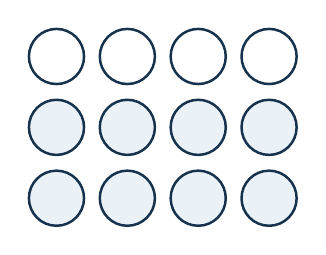
\begin{tikzpicture}[x=.9cm,y=.9cm]
\foreach \n in {0,...,11}{\pgfmathtruncatemacro{\x}{mod(\n,4)}\pgfmathtruncatemacro{\y}{floor(\n/4)}\ifnum\n<8\node[qra counter,fill=qraPale]at(\x,\y){};\else\node[qra counter,fill=white]at(\x,\y){};\fi}
\end{tikzpicture}\end{document}
